\maketitle

\newgeometry{margin=30mm,bmargin=50mm}%
\thispagestyle{empty}
\topskip=0pt
%
{%
\color{black!60!white}%
{\LARGE Them Bombs!}

\textsl{\Title}

\vspace{1em}

\Language\ \Version%
}%

\vspace{15mm}

\section*{注意!}

このマニュアルは\textit{Them Bombs!}の\textbf{PC, Mac, Linux,
Android Phone} (シングルタップ)\textbf{, iPhone, Nintendo Switch, Apple TV}版のみに適用されます。

マルチタッププラットフォーム (Android TabletまたはiPad)の場合は適切なマニュアルを\textsf{\url{https://www.thembombs.com/manual}}からダウンロードしてください。


\section*{はじめに}
マッドサイエンティストTiNT博士さまざまな公共場所に致命的な爆弾を仕掛けます。%
爆発の数分前、ランダムに選ばれた爆発範囲内の人は彼からメッセージを受け取ります。%
この人\~\textit{初心者ヒーロー}\~だけ爆弾を解除することができます… 適切な助言をもらった場合にですね。


\section*{ゲームのルール}
プレイヤーの中の一人が(\textit{Them Bombs!}ゲーム内で)爆弾を解除する\textit{初心者ヒーロー}になります。%
他のプレイヤーは\textit{エキスパートチーム}になり、このマニュアルを読めます。%
\textit{エキスパート}は\textit{ヒーロー}の画面を見れないし、\textit{ヒーロー}はこのマニュアルの内容を見てはいけません。

\textit{エキスパート}が\textit{ヒーロー}にラジオで話すように、プレイヤー全員は言葉だけでコミュニケーションをとります。

\vspace{1em}
成功の鍵は落ち着いて\textit{効率的なコミュニケーション}をすること、そしてこのマニュアルを\textit{よく読む}ことです。%

\vspace{1em}
あなたの生存を祈ります!

\newgeometry{margin=30mm,bmargin=35mm}%
\parskip=1em
\vspace*{-20mm}
\section*{TiNT博士の手口}
一つだけ確かなことは{、}TiNT博士は狂った男だということです… 彼はすべての地獄が解き放たれるのを楽しんでいるようです。

TiNT博士のデバイスは共通の設計を共有しています。%
起爆剤が付いている小さな爆弾と、それに接続された火薬が入っている大きなコンテナがあります。%
彼が爆発物をどこで入手したかは不明です。%
彼がどのように爆弾を運ぶかも謎です。%

確かなものもありますが…\\
コンテナを動かしてみたら……爆弾が爆発します!\\
開始爆弾を切り離してみたら……爆弾は爆発します!\\
タイマーのバッテリーを外してみたら……爆弾が爆発します!\\
起爆剤を取り除くようにしてみたら……爆弾が爆発します!\\
これらの教訓は、多くの\textit{ヒーロー}たちが苦労して学んだものです。%

これまでに証明された爆弾の解除の唯一の方法は、爆弾のセキュリティモジュールを解除することみたいです。%
セキュリティモジュールはTiNT博士の変態的なゲームの要素のようです。

通常{、}TiNT博士は潜在的な犠牲者の中の1人だけに追跡できないメッセージで警告を発します。%
彼はまた{、}まるで\textit{ヒーロー}が成功し悲劇を避けることを望んでいるかのように、いくつかの基本的な工具(電動ドライバー、ペンチ、懐中電灯など)を爆弾の後ろに隠しています。%

以前の事件の分析によると{、}TiNT博士に選択された人たりはいつも非常に勇敢な人たちだということが判明されました…

\newpage
\section*{TiNT博士の爆弾の解除\~その基礎}

爆弾を解除するには、セキュリティモジュールのすべての爆弾を無効にする必要があります。%
このマニュアルで全ての既知の爆弾の解除方法を説明しています。%

\textit{まず、ネジを緩めて爆弾のカバーを取り外します。(ご心配をおかけしますが、カバーは爆発する要素ではありません。)}

\vspace{1em}
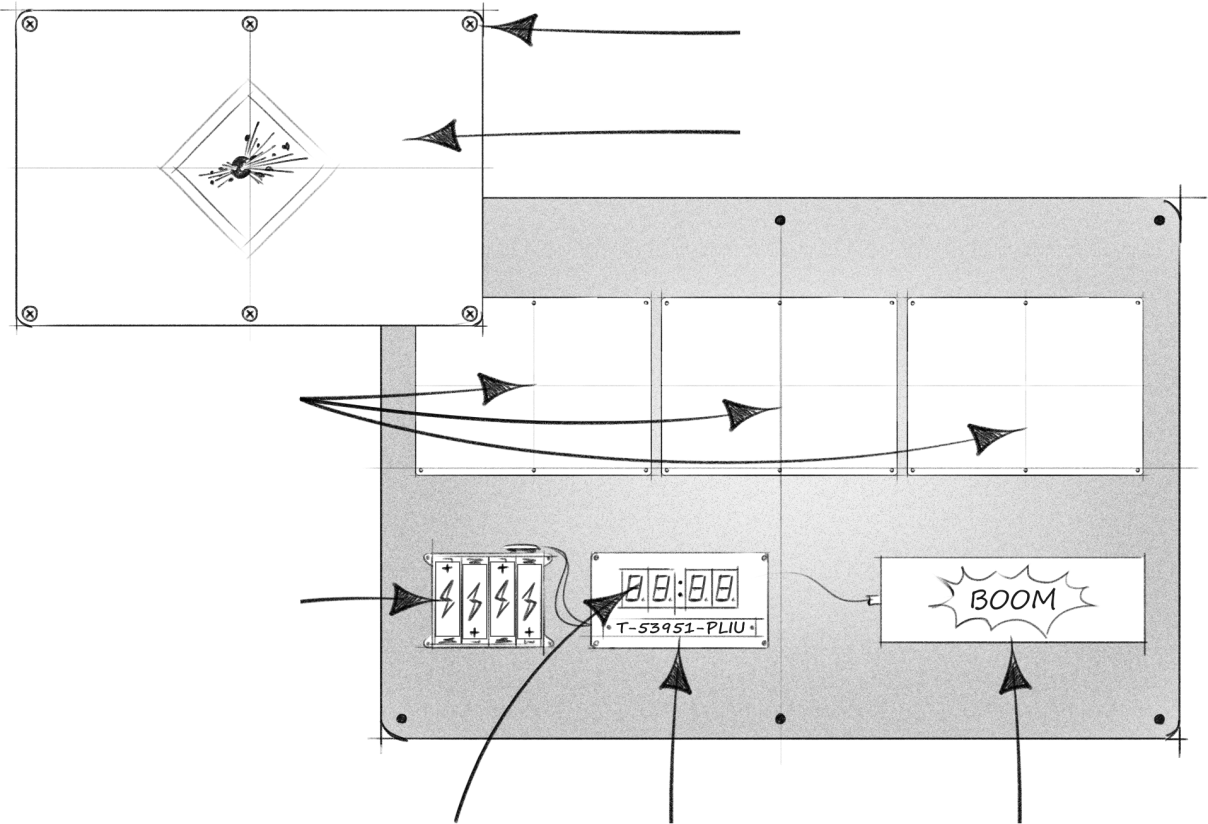
\includegraphics[width=\textwidth]{./images/2.png}

\begin{textblock*}{5cm}(12.5cm,8.6cm)
    \tegakifont カバー取り付けネジ
\end{textblock*}
\begin{textblock*}{5cm}(12.5cm,9.8cm)
    \tegakifont 爆弾のカバー
\end{textblock*}
\begin{textblock*}{5cm}(1.9cm,13.15cm)
    \tegakifont セキュリティモジュール
\end{textblock*}
\begin{textblock*}{5cm}(3.4cm,15.7cm)
    \tegakifont タイマーの電池
\end{textblock*}
\begin{textblock*}{5cm}(8cm,19cm)
    \tegakifont タイマー
\end{textblock*}
\begin{textblock*}{5cm}(9cm,19cm)
    \centering
    \tegakifont タイマーの\\シリアル番号
\end{textblock*}
\begin{textblock*}{5cm}(15cm,19cm)
    \tegakifont 起爆剤
\end{textblock*}


\newpage
\begin{minipage}{0.63\textwidth}
\parskip=1em
\section*{セキュリティモジュール:3つの点滅するボタン}

\uline{概要}:1文字のディスプレイと3つのカラフルな点滅ボタンがあります。

\uline{解除方法}:各ボタンが正しい色で点滅しているときにボタンを押します。
\end{minipage}%
\hfill%
\begin{minipage}{0.33\textwidth}
    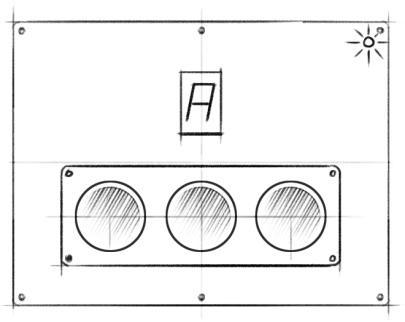
\includegraphics[width=\textwidth]{images/4.png}
    \vspace*{\fill}
\end{minipage}

正しい色のセットは、次のように決定されます。\\
1. ディスプレイに表示される文字(文字は定期的に変わります!)\\
2. 爆発までの残り時間。

下の表でライトの色の正しい組み合わせを見つけてください。

\uline{表の読み方}:縦線で区切られた3つの文字は{、}3つのボタンの色に対応しています。表示される色は次のとおりです。\\
\hspace*{6em} Y -- 黄\hspace*{3em}R -- 赤\hspace*{3em}B -- 青

例:Y|R|B -- \uline{黄、赤、青の順}で点滅する瞬間に各ボタンを押します。

\bgroup%
\def\arraystretch{1.5}
\fontsize{10.5}{13}\selectfont
\def\emphchar#1{\raisebox{-.1em}{\large\bfseries #1}}
\begin{tabular}{c|ccccccc|}
    \cline{2-8}
                                             & \multicolumn{7}{c|}{表示されている文字} \\ \hline
    \multicolumn{1}{|c|}{残り時間} & \emphchar{A} & \emphchar{B} & \emphchar{C} & \emphchar{D} & \emphchar{E} & \emphchar{F} & \emphchar{G} \\ \hline
    \multicolumn{1}{|c|}{240秒超過}            & Y|B|R & Y|R|Y & R|R|R & B|Y|B & B|B|B & R|Y|R & Y|Y|Y \\
    \multicolumn{1}{|c|}{120秒超過{、}240秒以下} & B|Y|B & B|R|B & B|B|Y & Y|Y|R & R|B|Y & R|Y|Y & Y|B|R \\
    \multicolumn{1}{|c|}{60秒超過{、}120秒以下}  & Y|Y|Y & B|B|B & R|Y|Y & Y|B|R & B|B|Y & B|R|B & Y|Y|R \\
    \multicolumn{1}{|c|}{60秒以下}         & R|R|R & B|B|Y & R|Y|R & R|B|Y & B|R|B & Y|R|Y & R|R|R \\ \hline
\end{tabular}%
\egroup

\begin{center}
    (240秒 = 4分, 120秒 = 2分, 60秒 = 1分)
\end{center}

「まだ生きている爆発物処理班」の為のヒント:
\begin{itemize}
    \item[$\bullet$] 最初の2つのボタンについては{、}正しい色を押すときに間違いを犯してもいいです。(シーケンスを続行するには{、}もう一度押すだけです。) ただし{、}3番目のボタンを押すときは{、}正しくないと不快な結果が生じます。
    \item[$\bullet$] とても難しい仕事に思えますか?黒と押したい色の間に現れる色の数を覚えてみてください。
\end{itemize}



\newpage
\begin{minipage}{0.63\textwidth}
    \parskip=1em
    \section*{セキュリティモジュール:15個のタイルと点滅するライト}
    
    \uline{概要}:15個のタイルと点滅するライト{、}OKボタンがあります。
    
    \uline{解除方法}:タイルを押して正しく光るようにしてOKボタンを押します。
\end{minipage}%
\hfill%
\begin{minipage}{0.33\textwidth}
    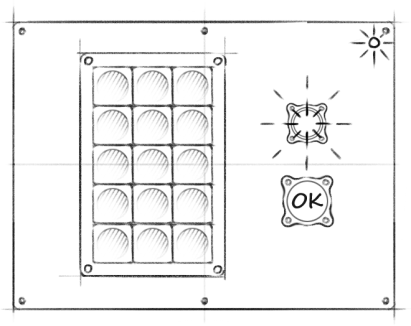
\includegraphics[width=\textwidth]{images/7.png}
    \vspace*{\fill}
\end{minipage}

点滅する光は、モールス符号を使用して文字または数字の信号を送信しています。付録IIIを参照してください。タイルを押してこの文字/数字の形を再現してください。

\uline{可能なタイルの組み合わせ}:

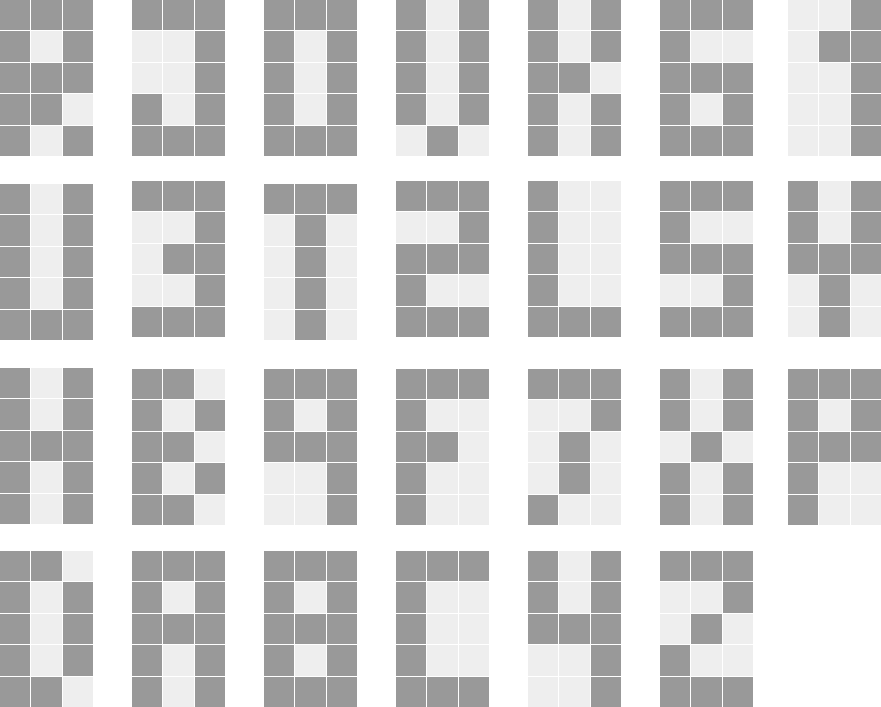
\includegraphics[width=\textwidth]{images/5.png}

\newpage
\begin{minipage}{0.63\textwidth}
    \parskip=1em
    \section*{セキュリティモジュール:5文字のコード}
    
    \uline{概要}:数字の並び{、}5文字のディスプレイ(上下の矢印を使用して文字を変更できます){、}および\hfill\\{[OK]}ボタンがある鉄板。
\end{minipage}%
\hfill%
\begin{minipage}{0.33\textwidth}
    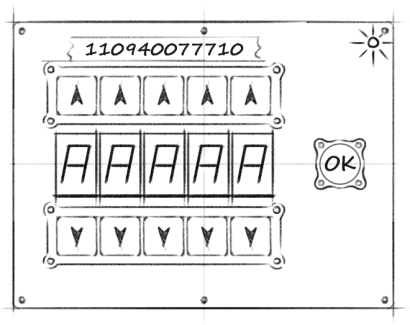
\includegraphics[width=\textwidth]{images/9.png}
    \vspace*{\fill}
\end{minipage}

\uline{解除方法}:正しい5文字のコードを入力し{、} {[OK]}を押します。\\
左から順番に数字を足していきます。偶数の桁になったら{、}足すのをやめます。(ただし{、}偶数の桁も足します。)下の表で結果を見つけてください。\\
残りの桁について{、}この過程を繰り返します。

例:\\
\hspace*{3em}1112の合計は5になり、文字Aに対応します。\\
\hspace*{3em}1112330は5と6になり、文字AとBに対応します。


\begin{center}
\large
\def\arraystretch{1.5}
\begin{tabular}{|l|l|l}
    \hline
    A - \ 5 \hspace*{1em}  & J - \ 17\hspace*{1em}  & \multicolumn{1}{l|}{S - \ 2\hspace*{1em} }   \\ \hline
    B - \ 6 \hspace*{1em}  & K - \ 21\hspace*{1em}  & \multicolumn{1}{l|}{T - \ 7\hspace*{1em} }   \\ \hline
    C - \ 27\hspace*{1em}  & L - \ 8 \hspace*{1em}  & \multicolumn{1}{l|}{U - \ 25\hspace*{1em} } \\ \hline
    D - \ 12\hspace*{1em}  & M - \ 14\hspace*{1em}  & \multicolumn{1}{l|}{V - \ 15\hspace*{1em} } \\ \hline
    E - \ 0 \hspace*{1em}  & N - \ 10\hspace*{1em}  & \multicolumn{1}{l|}{W - \ 16\hspace*{1em} } \\ \hline
    F - \ 11\hspace*{1em}  & O - \ 3 \hspace*{1em}  & \multicolumn{1}{l|}{X - \ 19\hspace*{1em} } \\ \hline
    G - \ 26\hspace*{1em}  & P - \ 22\hspace*{1em}  & \multicolumn{1}{l|}{Y - \ 20\hspace*{1em} } \\ \hline
    H - \ 13\hspace*{1em}  & Q - \ 18\hspace*{1em}  & \multicolumn{1}{l|}{Z - \ 24\hspace*{1em} } \\ \hline
    I - \ 4 \hspace*{1em}  & R - \ 9 \hspace*{1em}  &                             \\\cline{1-2}
\end{tabular}
\end{center}


「まだ生きている爆発物処理班」の為のヒント:
\begin{itemize}
    \item[$\bullet$] 数列にはちょうど5つの偶数があります。
    \item[$\bullet$] 「ゼロ」も偶数!
\end{itemize}


\newpage
\begin{minipage}{0.63\textwidth}
    \parskip=1em
    \section*{セキュリティモジュール:ピザ}
    
    \uline{概要}:8つの三角形があります。いくつかの三角形が順番通り光っています。

    \uline{解除方法}:すべての正しい三角形を押してください。回答入力欄は最初に三角形を押してから数えて{、}いつも約3\~6秒間有効になります。
\end{minipage}%
\hfill%
\begin{minipage}{0.33\textwidth}
    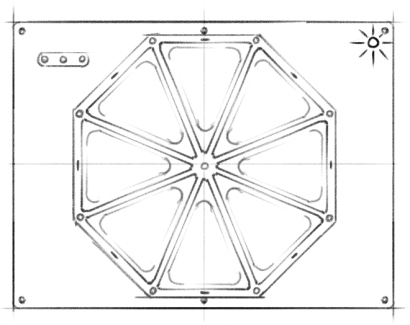
\includegraphics[width=\textwidth]{images/11.png}
    \vspace*{\fill}
\end{minipage}

\uline{押す三角形}:
\begin{itemize}
    \item[$\bullet$] 爆弾のカバーが4つのネジで取り付けられていた場合は{、}点灯した三角形のみを押します。{*}
    \item[$\bullet$] 爆弾のカバーが6つのネジで取り付けられていた場合は{、}点灯しなかった三角形のみを押してください。{*}
\end{itemize}
*以下の例外を参照してください。

\uline{例外}:
\begin{itemize}
    \item[$\bullet$] タイマーのバッテリーに二酸化マンガンリチウム電池が使用されている場合(付録Iを参照){、}北の三角形を押さないでください。
    \item[$\bullet$] 反対側になっているバッテリーホルダーが存在する場合(付録Iを参照){、}南の三角形を押さないでください。
    \item[$\bullet$] タイマーのシリアル番号に少なくとも1つの偶数が含まれている場合は{、}東の三角形を押さないでください。
    \item[$\bullet$] タイマーの通し番号が偶数のみの場合は{、}西の三角を押さないでください。
\end{itemize}

「まだ生きている爆発物処理班」の為のヒント:
\begin{itemize}
    \item[$\bullet$] ゼロも偶数です。
    \item[$\bullet$] 三角形を押して{、}組み合わせが承認または拒否されるまで待ちます。これは3\~6秒以内に行われます。
    \item[$\bullet$] 上記の指示に従ったら押す三角形がなくなった場合は{、}ランダムな三角形を2回押してください。
\end{itemize}


\newpage
\section*{セキュリティモジュール:電子錠}


\uline{概要}:対になっている赤と青の接続プレートでできているロックが5つあります。また5つの絞りと一つのスイッチがあります。

\begin{center}
    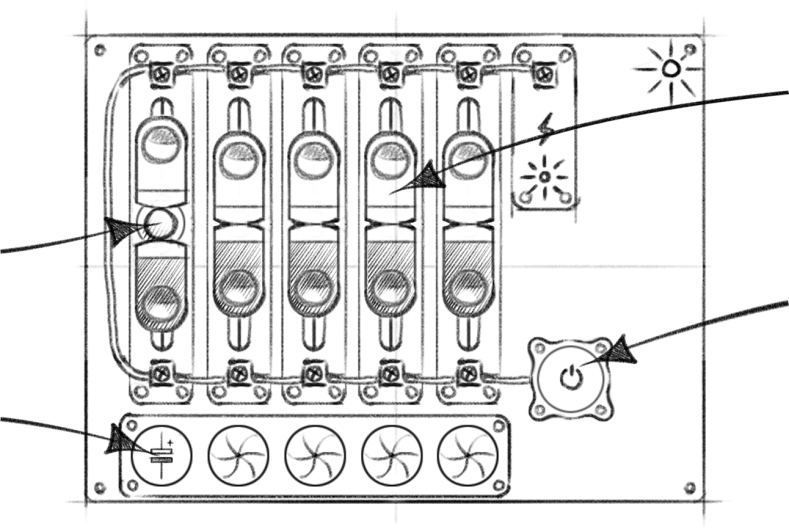
\includegraphics[width=0.6\textwidth]{images/13.png}
\end{center}

\begin{textblock*}{5cm}(2.6cm,9.1cm)
    \tegakifont インシュレータ
\end{textblock*}
\begin{textblock*}{5cm}(1.4cm,11cm)
    \tegakifont 記号が書いている絞り
\end{textblock*}
\begin{textblock*}{5cm}(15.5cm,7.3cm)
    \tegakifont ロック
\end{textblock*}
\begin{textblock*}{5cm}(15.5cm,9.8cm)
    \tegakifont スイッチ
\end{textblock*}


\uline{解除方法}:正しいロックを開き{、}モジュールに電流を流します。\\
ロックごとに{、}次の手順を1つずつ実行します。\\
\begin{enumerate}
    \item (青または赤の接続プレートをドラッグして)慎重にロックを開き{、}ロックの下の絞りが開きます。
    \item 次のページのリストのいずれかで記号を見つけます。
    \item 記号がロックが開いている必要があることを示している場合(断絶記号){、}ロックの接続プレートの間にインシュレータを配置し(接続プレート間の円を押します){、}次のロックに進みます。
    \item 記号がロックを閉じている必要があることを示している場合(連結記号){、}ロックを閉じて{、}次のロックに進みます。
\end{enumerate}

最後に{、}電源スイッチを押して電源を入れます。 正しいロックが開閉されている場合{、}モジュールは解除されます。

「まだ生きている爆発物処理班」の為のヒント:
\begin{itemize}
    \item[$\bullet$] ショートしないように注意!ロックの接続プレートを広げすぎたときにショートが発生します。
    \item[$\bullet$] 記号をよく見てください。誤解を招く可能性があります…
    \item[$\bullet$] 間違えた場合は{、}もう一度押してインシュレータを取り外すことができます。
\end{itemize}

\newpage

{\large 断絶記号:ロックが開いている必要があります。インシュレータを配置してください。}
\begin{center}
    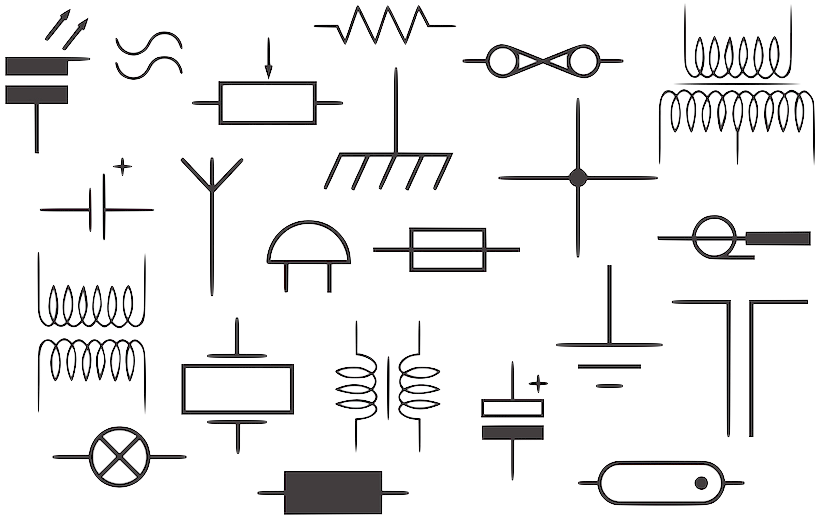
\includegraphics[width=\textwidth]{images/14.png}
\end{center}

{\large 連結記号:ロックが閉じている必要があります。}
\begin{center}
    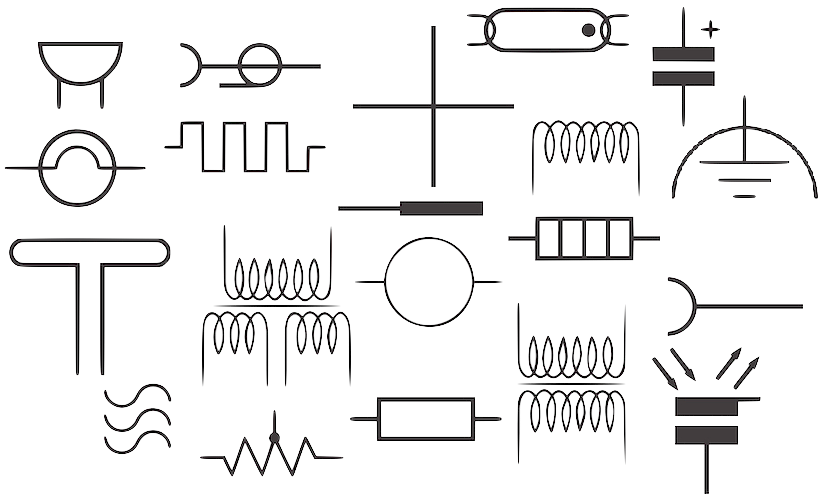
\includegraphics[width=\textwidth]{images/15.png}
\end{center}



\newpage
\begin{minipage}{0.63\textwidth}
    \parskip=1em
    \section*{セキュリティモジュール:4つの回転リング}
    
    \uline{概要}:4つの回転リングがあります。 各リングには、リングの向きを示す矢印が付いています。
    
    \uline{解除方法}:各リングを押して回転し、正しい基本方向に向けます。
\end{minipage}%
\hfill%
\begin{minipage}{0.33\textwidth}
    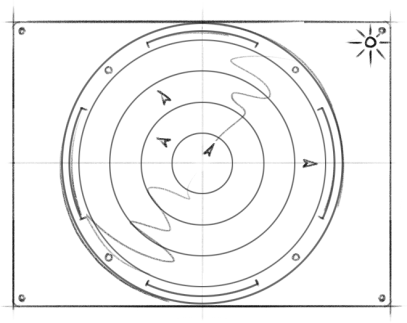
\includegraphics[width=\textwidth]{images/17.png}
    \vspace*{\fill}
\end{minipage}

\hspace*{3em}N - 北\hspace*{3em}W - 西\\
\hspace*{3em}S - 南\hspace*{3em}E - 東

方位は、リングの外側の境界に表示されています。

\uline{指示ポイントの読み方}:タイマーの電池、タイマーのシリアル番号、爆弾のカバーなど、爆弾の重要な要素を確認してください。 次に、下の表で正しい方位を見つけます。


\bgroup
\fontsize{9}{9}\selectfont
\def\arraystretch{1.4}
\begin{tabular}{|c|l|}
\hline
リング &
\multicolumn{1}{c|}{正しい方位} \\ \hline
1(一番大きいリング) &
\parbox{0.7\textwidth}{
    \vspace*{0.5em}
    付録Iでタイマーの電池電圧を確認してください。
    \vspace*{0.5em}
    \begin{itemize}
        \item[$\bullet$] 合計電圧が9 Vを超える場合 -- N
        \item[$\bullet$] 合計電圧が8 Vの場合 -- S
        \item[$\bullet$] 合計電圧が2.6 Vを超える場合 -- W
        \item[$\bullet$] その他の場合 -- E
    \end{itemize}
    \vspace*{1em}
} \\ \hline
2 &
\parbox{0.7\textwidth}{
    \vspace*{0.5em}
    タイマーの隣のタイマーシリアル番号を確認してください。
    \begin{itemize}
        \item[$\bullet$] シリアル番号の頭文字がYの場合 -- N
        \item[$\bullet$] シリアル番号の頭文字がTの場合 -- S
        \item[$\bullet$] シリアル番号の頭文字がAの場合 -- W
        \item[$\bullet$] その他の場合 -- E
    \end{itemize}
    \vspace*{1em}
} \\ \hline
3 &
\parbox{0.7\textwidth}{
    \vspace*{0.5em}
    付録Iでタイマーの電池セルの種類を確認してください。
    \vspace*{0.5em}
    \begin{itemize}
        \item[$\bullet$] 酸化銀電池の場合 -- N
        \item[$\bullet$] 二酸化マンガンリチウム電池の場合 -- S
        \item[$\bullet$] 二酸化マンガン亜鉛電池の場合 -- W
        \item[$\bullet$] その他の場合 -- E
    \end{itemize}
    \vspace*{1em}
} \\ \hline
4(一番小さいリング) &
\parbox{0.7\textwidth}{
    \vspace*{0.5em}
    爆弾のカバーの色が
    \vspace*{0.5em}
    \begin{itemize}
        \item[$\bullet$] 緑 -- N
        \item[$\bullet$] 赤 -- S
        \item[$\bullet$] 青 -- W
        \item[$\bullet$] その他の場合 -- E
    \end{itemize}
    \vspace*{1em}
} \\ \hline
\end{tabular}
\egroup

「まだ生きている爆発物処理班」の為のヒント:
\begin{itemize}
    \item[$\bullet$] 間違えても心配いりません。もう一度リングを押して再起動してください。
    \item[$\bullet$] リングが基点の1つに停止すると、リングの矢印が黄色に点灯します。
\end{itemize}


\newpage
\begin{minipage}{0.63\textwidth}
    \parskip=1em
    \section*{セキュリティモジュール:トラップ}
    
    \uline{概要}:押したくなるテキストが書いている大きなボタンがあります。例えば{、}

    \begin{itemize}
        \item Click me!(私を押してください!),
        \item Press here!(ここを押してください!),
        \item Click to defuse!(押して爆弾を解除しましょう!)
    \end{itemize}
    
    などです。
\end{minipage}%
\hfill%
\begin{minipage}{0.33\textwidth}
    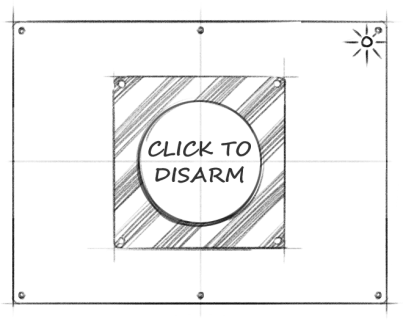
\includegraphics[width=\textwidth]{images/19.png}
    \vspace*{\fill}
\end{minipage}
    
\uline{注意!}:このボタンを不用意に押してはいけません。これはトラップです。爆弾はその瞬間に爆発します。
    
\uline{解除方法}:このセキュリティモジュールは必ず最後に解除してください。他のすべてのセキュリティモジュールが解除されたら、ボタンを3秒以上押し続けてから離します。

「まだ生きている爆発物処理班」の為のヒント:
\begin{itemize}
    \item 気をつけてください!エラーの余地はありません!
\end{itemize}


\newpage
\begin{minipage}{0.63\textwidth}
    \parskip=1em
    \section*{セキュリティモジュール:ワイヤー}
    
    \uline{概要}:垂直に取り付けられた3\string~6個の色分けされたワイヤー。 各ワイヤは{、}"+"および"-"とマークされた接触プレートに接続されています。
    
    \uline{解除方法}:右の接触プレート("+"と"-")どっちかの中で正しいものを押してから、正しいワイヤーを切断します。
\end{minipage}%
\hfill%
\begin{minipage}{0.33\textwidth}
    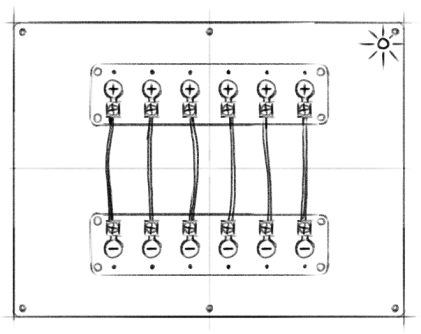
\includegraphics[width=\textwidth]{images/21.png}
    \vspace*{\fill}
\end{minipage}

この爆弾に使用されている起爆剤の種類を付録IIを参照し確認してください。\\
起爆剤が\uline{\textbf{C-4}、\textbf{Semtex}、または\textbf{TNT}}の場合は、表Aを参照してください。\\
起爆剤が\uline{ダイナマイト、即席爆発物、またはその他}の場合は、表Bを参照してください。

\bgroup
\def\arraystretch{1.3}
\begin{tabular}{|l|}\hline
表{A}({C-4}、{Semtex}、{TNT})\\\hline
\parbox{\textwidth}{
\vspace*{0.3em}
- ワイヤーが3本あり、すべて同じ色の場合は、左側のワイヤーの[+]と右側のワイヤーの[-]を押します。そして真ん中のワイヤーを切断します。\\[0.5em]
- 3本または4本のワイヤーがあり、そのうちの2本が青色の場合は、右側の青色のワイヤーの[+]と左側の青色のワイヤーの[-]を押します。すべてのワイヤーを切断します。\\[0.5em]
- 3本または4本のワイヤーがあり、そのうちの2本だけが黄色の場合は、両方の黄色のワイヤーの[+]と黄色のワイヤーの間のワイヤーの[-]を押します。黄色のワイヤーのみ切ります。\\[0.5em]
- 5本のワイヤーがあり、そのうち3本が同じ色の場合は、右から一番目のワイヤーの[+]と左から一番目のワイヤーの[-]を押します。すべてのワイヤーを切ります。\\[0.5em]
- 5本のワイヤーがあり、そのうち2本が赤色の場合は、両方の赤色のワイヤーの[+]と右から一番目のワイヤーの[-]を押します。赤い線以外すべて切ります。\\[0.5em]
- 5本のワイヤーがあり、そのうち2本が緑色の場合は、両方の緑色のワイヤーの[+]と左から一番目のワイヤーの[-]を押します。すべてのワイヤーを切断します。
\vspace*{0.3em}
}\\\hline
\end{tabular}
\egroup

\bgroup
\def\arraystretch{1.3}
\begin{tabular}{|l|}\hline
表{B}(ダイナマイト、即席爆発物、その他)\\\hline
\parbox{\textwidth}{
\vspace*{0.3em}
- ワイヤーが3本あり、すべて同じ色の場合は、右側のワイヤーの[+]と左側のワイヤーの[-]を押します。真ん中のワイヤーを切断します。\\[0.5em]
- 3本または4本のワイヤーがあり、そのうちの2本が青色の場合は、左側の青色のワイヤーの[+]と右側の青色のワイヤーの[-]を押します。すべてのワイヤーを切断します。\\[0.5em]
- 3本または4本のワイヤーがあり、そのうちの2本だけが黄色の場合は、両方の黄色のワイヤーの[-]と黄色のワイヤーの間のワイヤーの[+]を押します。黄色のワイヤーのみ切ります。\\[0.5em]
- 5本のワイヤーがあり、そのうち3本が同じ色の場合は、左から一番目のワイヤーの[+]と右から一番目のワイヤーの[-]を押します。すべてのワイヤーを切ります。\\[0.5em]
- 5本のワイヤーがあり、そのうち2本が赤色の場合は、両方の赤色のワイヤーの[+]と左から一番目のワイヤーの[-]を押します。赤いワイヤー以外すべて切ります。\\[0.5em]
- 5本のワイヤーがあり、そのうち2本が緑色の場合は、両方の緑色のワイヤーの[-]と左から一番目のワイヤーの[+]を押します。すべてのワイヤーを切断します。
\vspace*{0.3em}
}\\\hline
\end{tabular}
\egroup

\vspace*{2em}

「まだ生きている爆発物処理班」の為のヒント:
\begin{itemize}
    \item[$\bullet$] ワイヤーの色は、赤、青、緑、ピンク、黄、または茶色のみです。
    \item[$\bullet$] 間違ったワイヤーを切断すると、すぐに爆発したり、カウントダウン時間が大幅に短縮されたりする可能性があります。
    \item[$\bullet$] 時間の浪費を避けるために、ワイヤーを切断する前に、正しい接触プレート(および正しい接触プレートのみ!)が押されていることを確認してください。
\end{itemize}



\newpage
\begin{minipage}{0.63\textwidth}
    \parskip=1em
    \section*{セキュリティモジュール:3重安全装置}
    
    \uline{概要}:12個の丸い色分けされたボタンとギリシャ語のアルファベットの文字が付いたシャッター、有名な科学者の名前が書いております。
    
    \uline{解除方法}:連続する2つの鍵をそれぞれ開き、正しい4桁のコードを入力します。
\end{minipage}%
\hfill%
\begin{minipage}{0.33\textwidth}
    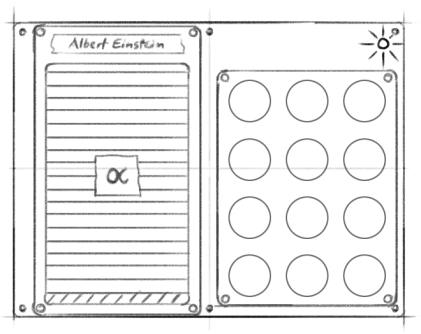
\includegraphics[width=\textwidth]{images/31.png}
    \vspace*{\fill}
\end{minipage}

\uline{A. 一つ目の鍵}:色分けされたボタンの正しい組み合わせを押します。\\
組み合わせは次のように決定されます。\\
\hspace*{1em}1. シャッターに見えるギリシャ文字、\\
\hspace*{1em}2. 科学者の名前。\\
次の表に可能な組み合わせを示します。\\
ボタンの数と色が正しければ、どのボタンを押してもかまいません。

\bgroup
\def\arraystretch{1.3}
\fontsize{9.5}{11}\selectfont
\begin{tabular}{c|cccccccc|}
\cline{2-9}
    &
    \multicolumn{8}{c|}{シャッターに付いているギリシャ文字} \\ \hline
\multicolumn{1}{|c|}{科学者} &
    \multicolumn{1}{c|}{\vphantom{\Huge A}\scalebox{2}{$\alpha$}} &
    \multicolumn{1}{c|}{\vphantom{\Huge A}\scalebox{2}{$\beta$}} &
    \multicolumn{1}{c|}{\vphantom{\Huge A}\scalebox{2}{$\gamma$}} &
    \multicolumn{1}{c|}{\vphantom{\Huge A}\scalebox{2}{$\delta$}} &
    \multicolumn{1}{c|}{\vphantom{\Huge A}\scalebox{2}{$\varepsilon$}} &
    \multicolumn{1}{c|}{\vphantom{\Huge A}\scalebox{2}{$\zeta$}} &
    \multicolumn{1}{c|}{\vphantom{\Huge A}\scalebox{2}{$\eta$}} &
    \multicolumn{1}{c|}{\vphantom{\Huge A}\scalebox{2}{$\theta$}} \\ \hline
\multicolumn{1}{|c|}{\begin{tabular}[c]{@{}c@{}}Albert Einstein\\ 1879-1955\end{tabular}} &
    \multicolumn{1}{c|}{\begin{tabular}[c]{@{}c@{}}1Y 2G\\ 1R\end{tabular}} &
    \multicolumn{1}{c|}{2Y 2G} &
    \multicolumn{1}{c|}{1G 3R} &
    \multicolumn{1}{c|}{3Y 1R} &
    \multicolumn{1}{c|}{4G} &
    \multicolumn{1}{c|}{4R} &
    \multicolumn{1}{c|}{4Y} &
    \begin{tabular}[c]{@{}c@{}}1Y 1G\\ 2R\end{tabular} \\ \hline
\multicolumn{1}{|c|}{\begin{tabular}[c]{@{}c@{}}Isaac Newtwon\\ 1643-1727\end{tabular}} &
    \multicolumn{1}{c|}{4G} &
    \multicolumn{1}{c|}{4R} &
    \multicolumn{1}{c|}{2Y 2R} &
    \multicolumn{1}{c|}{1G 3R} &
    \multicolumn{1}{c|}{2G 2R} &
    \multicolumn{1}{c|}{\begin{tabular}[c]{@{}c@{}}1Y 2G\\ 1R\end{tabular}} &
    \multicolumn{1}{c|}{3Y 1G} &
    3Y 1R \\ \hline
\multicolumn{1}{|c|}{\begin{tabular}[c]{@{}c@{}}Marie Curie\\ 1867-1934\end{tabular}} &
    \multicolumn{1}{c|}{2Y 2G} &
    \multicolumn{1}{c|}{1Y 3R} &
    \multicolumn{1}{c|}{\begin{tabular}[c]{@{}c@{}}2Y 1G\\ 1R\end{tabular}} &
    \multicolumn{1}{c|}{1Y 3G} &
    \multicolumn{1}{c|}{3Y 1R} &
    \multicolumn{1}{c|}{2G 2R} &
    \multicolumn{1}{c|}{4R} &
    3G 1R \\ \hline
\multicolumn{1}{|c|}{\begin{tabular}[c]{@{}c@{}}Louis Pasteur\\ 1822-1895\end{tabular}} &
    \multicolumn{1}{c|}{2Y 2R} &
    \multicolumn{1}{c|}{\begin{tabular}[c]{@{}c@{}}1Y 2G\\ 1R\end{tabular}} &
    \multicolumn{1}{c|}{4R} &
    \multicolumn{1}{c|}{3Y 1G} &
    \multicolumn{1}{c|}{1G 3R} &
    \multicolumn{1}{c|}{\begin{tabular}[c]{@{}c@{}}2Y 1G\\ 1R\end{tabular}} &
    \multicolumn{1}{c|}{2Y 2G} &
    4Y \\ \hline
\multicolumn{1}{|c|}{\begin{tabular}[c]{@{}c@{}}Nikola Tesla\\ 1856-1943\end{tabular}} &
    \multicolumn{1}{c|}{2G 2R} &
    \multicolumn{1}{c|}{\begin{tabular}[c]{@{}c@{}}2Y 1G\\ 1R\end{tabular}} &
    \multicolumn{1}{c|}{3Y 1R} &
    \multicolumn{1}{c|}{4Y} &
    \multicolumn{1}{c|}{1Y 3G} &
    \multicolumn{1}{c|}{\begin{tabular}[c]{@{}c@{}}1Y 1G\\ 2R\end{tabular}} &
    \multicolumn{1}{c|}{3G 1R} &
    4G \\ \hline
\multicolumn{1}{|c|}{\begin{tabular}[c]{@{}c@{}}Thomas Edison\\ 1847-1931\end{tabular}} &
    \multicolumn{1}{c|}{4R} &
    \multicolumn{1}{c|}{4Y} &
    \multicolumn{1}{c|}{4G} &
    \multicolumn{1}{c|}{1Y 3R} &
    \multicolumn{1}{c|}{2Y 2G} &
    \multicolumn{1}{c|}{3G 1R} &
    \multicolumn{1}{c|}{2Y 2R} &
    1G 3R \\ \hline
\multicolumn{1}{|c|}{\begin{tabular}[c]{@{}c@{}}Blasie Pascal\\ 1623-1662\end{tabular}} &
    \multicolumn{1}{c|}{1G 3R} &
    \multicolumn{1}{c|}{2G 2R} &
    \multicolumn{1}{c|}{\begin{tabular}[c]{@{}c@{}}1Y 1G\\ 2R\end{tabular}} &
    \multicolumn{1}{c|}{2Y 2R} &
    \multicolumn{1}{c|}{3Y 1G} &
    \multicolumn{1}{c|}{1Y 3R} &
    \multicolumn{1}{c|}{\begin{tabular}[c]{@{}c@{}}1Y 1G\\ 2R\end{tabular}} &
    1Y 3G \\ \hline
\multicolumn{1}{|c|}{\begin{tabular}[c]{@{}c@{}}Galileo Galilei\\ 1564-1642\end{tabular}} &
    \multicolumn{1}{c|}{3Y 1G} &
    \multicolumn{1}{c|}{2Y 2G} &
    \multicolumn{1}{c|}{1Y 3G} &
    \multicolumn{1}{c|}{4G} &
    \multicolumn{1}{c|}{\begin{tabular}[c]{@{}c@{}}2Y 1G\\ 1R\end{tabular}} &
    \multicolumn{1}{c|}{3Y 1R} &
    \multicolumn{1}{c|}{\begin{tabular}[c]{@{}c@{}}1Y 2G\\ 1R\end{tabular}} &
    1Y 3R \\ \hline
\end{tabular}
\egroup

\begin{center}
    Y -- 黄\qquad G -- 緑\qquad R -- 赤
\end{center}

例:1Y 2G 1Rの組み合わせの場合{、}次のボタンを押します。
\begin{center}
    黄色のボタン1つ{、}緑色のボタン2つ{、}赤色のボタン1つ。
\end{center}

\newpage

\uline{B. 二つ目の鍵}:ギリシャ文字が書かれた6つの四角いボタンのうち3つを押します。 正しい組み合わせは、次のように決定されます。\\
\hspace*{1em}1. 2番目のシャッター(6つの四角いボタンの下のドア)の色、\\
\hspace*{1em}2. 見えるギリシャ文字のセット。\\
以下の可能な組み合わせの1つだけが{、}爆弾モジュールの組み合わせと一致します。


\begin{center}
\def\makecell#1#2#3{\vphantom{\Huge A}\scalebox{1.5}{$\>{#1}\quad{#2}\quad{#3}\>$}}
\def\arraystretch{1.5}
\fontsize{10.5}{11}\selectfont
\begin{tabular}{c|cccc|}
\cline{2-5}
                            & \multicolumn{4}{c|}{可能な組み合わせ}                                            \\ \hline
\multicolumn{1}{|c|}{シャッターの色} & \multicolumn{1}{c|}{組み合わせ} & \multicolumn{1}{c|}{組み合わせ} & \multicolumn{1}{c|}{組み合わせ} & 組み合わせ \\ \hline
\multicolumn{1}{|c|}{青}  & 
\multicolumn{1}{c|}{\makecell{\alpha}{\delta}{\zeta}} & 
\multicolumn{1}{c|}{\makecell{\gamma}{\varepsilon}{\varkappa}} & 
\multicolumn{1}{c|}{\makecell{\beta}{\eta}{\psi}} & 
                    \makecell{\pi}{\mu}{\theta} \\ \hline
\multicolumn{1}{|c|}{灰色} & 
\multicolumn{1}{c|}{\makecell{\varrho}{\delta}{\varkappa}} & 
\multicolumn{1}{c|}{\makecell{\alpha}{\eta}{\zeta}} & 
\multicolumn{1}{c|}{\makecell{\iota}{\xi}{\lambda}} & 
                    \makecell{\psi}{\nu}{\mu} \\ \hline
\multicolumn{1}{|c|}{紫}  & 
\multicolumn{1}{c|}{\makecell{\tau}{\xi}{\beta}} & 
\multicolumn{1}{c|}{\makecell{\eta}{\iota}{\nu}} & 
\multicolumn{1}{c|}{\makecell{\delta}{\lambda}{\upsilon}} & 
                    \makecell{\varrho}{\omega}{\varepsilon} \\ \hline
\multicolumn{1}{|c|}{茶色} & 
\multicolumn{1}{c|}{\makecell{\sigma}{\gamma}{\varkappa}} & 
\multicolumn{1}{c|}{\makecell{\theta}{\zeta}{\pi}} & 
\multicolumn{1}{c|}{\makecell{\beta}{o}{\nu}} & 
                    \makecell{\omega}{\mu}{\alpha} \\ \hline
\multicolumn{1}{|c|}{橙色} & 
\multicolumn{1}{c|}{\makecell{\iota}{\nu}{o}} & 
\multicolumn{1}{c|}{\makecell{\lambda}{\gamma}{\sigma}} & 
\multicolumn{1}{c|}{\makecell{\chi}{\varepsilon}{\pi}} & 
                    \makecell{\psi}{\varrho}{\theta} \\ \hline
\end{tabular}
\end{center}

\uline{C. 4桁コード}:矢印を使用して数字を変更します。 正しいコードはその科学者が亡くなった年です。


\newpage
\begin{minipage}{0.63\textwidth}
    \parskip=1em
    \section*{セキュリティモジュール:音楽記号}
    
    \uline{概要}:音楽記号が書かれている5つの板とその上にモールス符号が書かれた紙があります。記号は上下の矢印を使用して変更できます。
\end{minipage}%
\hfill%
\begin{minipage}{0.33\textwidth}
    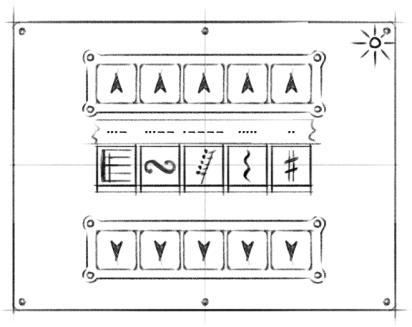
\includegraphics[width=\textwidth]{images/54.png}
    \vspace*{\fill}
\end{minipage}
    
\uline{解除方法}:各板を正しい音楽記号に設定します。\\付録IIIを参照して各モールス符号を文字または数字に変換します。次に{、}この文字または数字を下で見つけて{、}対応する記号を設定します。

モジュールは{、}5つの記号すべてに正しく設定してから3秒後に解除されます。

\begin{center}
    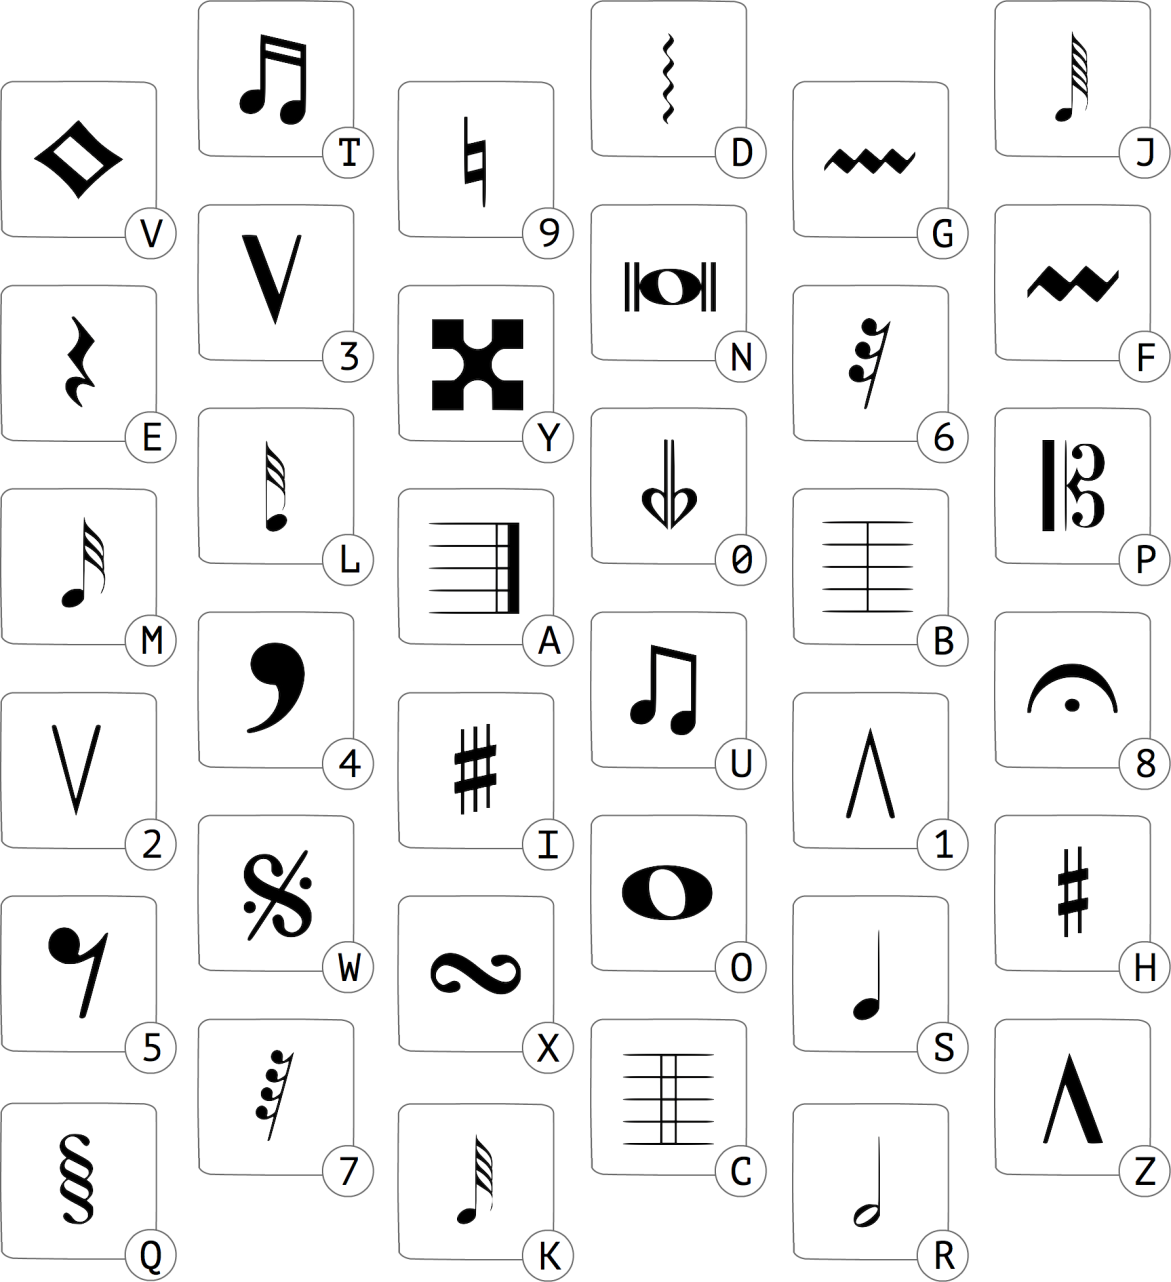
\includegraphics[width=0.85\textwidth]{images/52.png}
\end{center}


\newpage
\begin{minipage}{0.63\textwidth}
    \parskip=1em
    \section*{セキュリティモジュール:24個の点}
    
    \uline{概要}:左側に24個の丸いボタンと右側にディスプレイ一つと4つの色分けボタンがあります。
\end{minipage}%
\hfill%
\begin{minipage}{0.33\textwidth}
    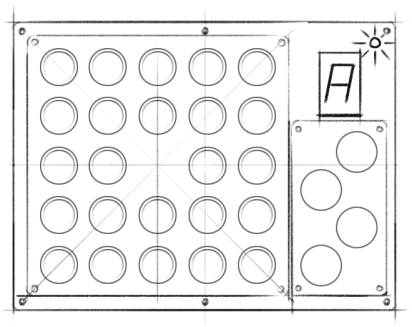
\includegraphics[width=\textwidth]{images/62.png}
    \vspace*{\fill}
\end{minipage}
\uline{解除方法}:正しい色を使用して、下の図に従って9つの丸いボタンを光らせます。
クエスチョンマーク(?)から始めて、矢印に従って連続するボックスに進みます。
ディスプレイ上の文字は次の2つを示します。
\begin{enumerate}
    \item 正しいパターンボックスを見つけるためにたどる矢印、
    \item 光らせる丸いボタンの色(表を参照)
\end{enumerate}

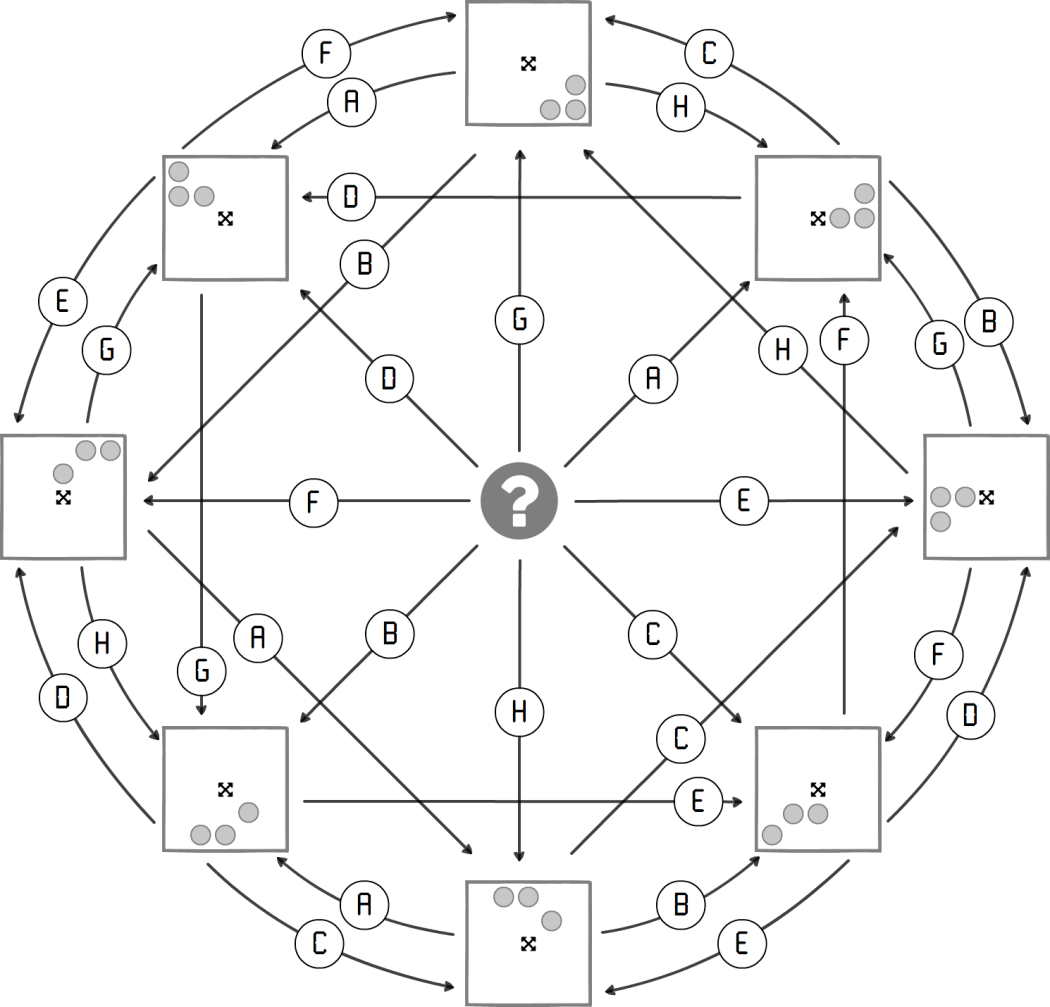
\includegraphics[width=0.78\textwidth]{images/55.png}

「まだ生きている爆発物処理班」の為のヒント:
\begin{itemize}
    \item[$\bullet$] 丸いボタンに色を付けるには、まず右側の色分けボタンを押してから、点灯させたい左側のボタンを押します。
    \item[$\bullet$] 上書きすることで色を変えることができます。色を完全に削除するには、色分けボタンが選択されていない状態で左側のボタンを押してください。色が変更できない場合は、その色が正しいことが既に確認されていることを意味します。
\end{itemize}

\begin{textblock*}{5cm}(16cm,18cm)
\bgroup
\def\arraystretch{1.4}
\begin{tabular}{|c|c|}
    \hline
    文字 & 色 \\ \hline
    A\quad E & 青 \\ \hline
    B\quad F & 黄 \\ \hline
    C\quad G & 赤 \\ \hline
    D\quad H & 緑 \\ \hline
\end{tabular}
\egroup
\end{textblock*}




\newpage
\begin{minipage}{0.63\textwidth}
    \parskip=1em
    \section*{セキュリティモジュール:3つのダイヤル}
    
    \uline{概要}:A, B, Cと表示されている3つのダイヤルと一文字のディスプレイ、そしてOKボタンがあります。

    \uline{解除方法}:3つのダイヤルを正しい数字を指すように回してOKボタンを押してください。
\end{minipage}%
\hfill%
\begin{minipage}{0.33\textwidth}
    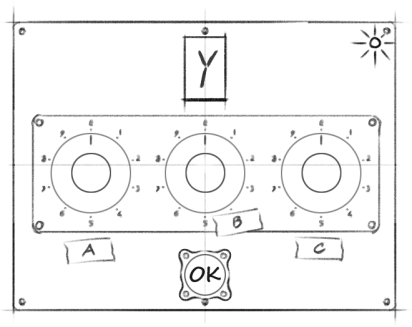
\includegraphics[width=\textwidth]{images/64.png}
    \vspace*{\fill}
\end{minipage}

\uline{ダイヤルA}:ダイヤルを回して、音が再生される値と、文字ディスプレイに「{X}」が表示される値を観察します。

\bgroup
\fontsize{9.5}{9.5}\selectfont
\begin{tabular}{|p{0.3\textwidth}p{0.3\textwidth}p{0.3\textwidth}|}
    \hline
    \multicolumn{3}{|c|}{ダイヤルA}\\ \hline
    \multicolumn{1}{|>{\centering}p{0.3\textwidth}|}{音が鳴る値} &
    \multicolumn{1}{|>{\centering}p{0.3\textwidth}|}{「{X}」が表示される値} &
    \multicolumn{1}{|>{\centering}p{0.3\textwidth}|}{正しいダイヤルAの値} \\ \hline
    \multicolumn{1}{|>{\centering}p{0.3\textwidth}|}{2} &
    \multicolumn{1}{|>{\centering}p{0.3\textwidth}|}{5} &
    \multicolumn{1}{|>{\centering}p{0.3\textwidth}|}{1} \\ \hline
    \multicolumn{1}{|>{\centering}p{0.3\textwidth}|}{2} &
    \multicolumn{1}{|>{\centering}p{0.3\textwidth}|}{3} &
    \multicolumn{1}{|>{\centering}p{0.3\textwidth}|}{2} \\ \hline
    \multicolumn{1}{|>{\centering}p{0.3\textwidth}|}{2} &
    \multicolumn{1}{|>{\centering}p{0.3\textwidth}|}{6} &
    \multicolumn{1}{|>{\centering}p{0.3\textwidth}|}{3} \\ \hline
    %
    \multicolumn{1}{|>{\centering}p{0.3\textwidth}|}{4} &
    \multicolumn{1}{|>{\centering}p{0.3\textwidth}|}{8} &
    \multicolumn{1}{|>{\centering}p{0.3\textwidth}|}{4} \\ \hline
    \multicolumn{1}{|>{\centering}p{0.3\textwidth}|}{4} &
    \multicolumn{1}{|>{\centering}p{0.3\textwidth}|}{7} &
    \multicolumn{1}{|>{\centering}p{0.3\textwidth}|}{5} \\ \hline
    %
    \multicolumn{1}{|>{\centering}p{0.3\textwidth}|}{6} &
    \multicolumn{1}{|>{\centering}p{0.3\textwidth}|}{0} &
    \multicolumn{1}{|>{\centering}p{0.3\textwidth}|}{6} \\ \hline
    \multicolumn{1}{|>{\centering}p{0.3\textwidth}|}{6} &
    \multicolumn{1}{|>{\centering}p{0.3\textwidth}|}{1} &
    \multicolumn{1}{|>{\centering}p{0.3\textwidth}|}{7} \\ \hline
    %
    \multicolumn{1}{|>{\centering}p{0.3\textwidth}|}{7} &
    \multicolumn{1}{|>{\centering}p{0.3\textwidth}|}{3} &
    \multicolumn{1}{|>{\centering}p{0.3\textwidth}|}{8} \\ \hline
    \multicolumn{1}{|>{\centering}p{0.3\textwidth}|}{7} &
    \multicolumn{1}{|>{\centering}p{0.3\textwidth}|}{6} &
    \multicolumn{1}{|>{\centering}p{0.3\textwidth}|}{9} \\ \hline
    \multicolumn{1}{|>{\centering}p{0.3\textwidth}|}{7} &
    \multicolumn{1}{|>{\centering}p{0.3\textwidth}|}{1} &
    \multicolumn{1}{|>{\centering}p{0.3\textwidth}|}{0} \\ \hline
    %
    \multicolumn{1}{|>{\centering}p{0.3\textwidth}|}{1} &
    \multicolumn{1}{|>{\centering}p{0.3\textwidth}|}{3} &
    \multicolumn{1}{|>{\centering}p{0.3\textwidth}|}{1} \\ \hline
    \multicolumn{1}{|>{\centering}p{0.3\textwidth}|}{1} &
    \multicolumn{1}{|>{\centering}p{0.3\textwidth}|}{7} &
    \multicolumn{1}{|>{\centering}p{0.3\textwidth}|}{2} \\ \hline
    \multicolumn{1}{|>{\centering}p{0.3\textwidth}|}{1} &
    \multicolumn{1}{|>{\centering}p{0.3\textwidth}|}{9} &
    \multicolumn{1}{|>{\centering}p{0.3\textwidth}|}{3} \\ \hline
    %
    \multicolumn{1}{|>{\centering}p{0.3\textwidth}|}{3} &
    \multicolumn{1}{|>{\centering}p{0.3\textwidth}|}{1} &
    \multicolumn{1}{|>{\centering}p{0.3\textwidth}|}{4} \\ \hline
    \multicolumn{1}{|>{\centering}p{0.3\textwidth}|}{3} &
    \multicolumn{1}{|>{\centering}p{0.3\textwidth}|}{5} &
    \multicolumn{1}{|>{\centering}p{0.3\textwidth}|}{5} \\ \hline
    %
    \multicolumn{1}{|>{\centering}p{0.3\textwidth}|}{5} &
    \multicolumn{1}{|>{\centering}p{0.3\textwidth}|}{8} &
    \multicolumn{1}{|>{\centering}p{0.3\textwidth}|}{6} \\ \hline
    \multicolumn{1}{|>{\centering}p{0.3\textwidth}|}{5} &
    \multicolumn{1}{|>{\centering}p{0.3\textwidth}|}{2} &
    \multicolumn{1}{|>{\centering}p{0.3\textwidth}|}{7} \\ \hline
    %
    \multicolumn{1}{|>{\centering}p{0.3\textwidth}|}{8} &
    \multicolumn{1}{|>{\centering}p{0.3\textwidth}|}{4} &
    \multicolumn{1}{|>{\centering}p{0.3\textwidth}|}{8} \\ \hline
    \multicolumn{1}{|>{\centering}p{0.3\textwidth}|}{8} &
    \multicolumn{1}{|>{\centering}p{0.3\textwidth}|}{0} &
    \multicolumn{1}{|>{\centering}p{0.3\textwidth}|}{9} \\ \hline
    %
    \multicolumn{1}{|>{\centering}p{0.3\textwidth}|}{9} &
    \multicolumn{1}{|>{\centering}p{0.3\textwidth}|}{7} &
    \multicolumn{1}{|>{\centering}p{0.3\textwidth}|}{0} \\ \hline
\end{tabular}
\egroup

\uline{ダイヤルB}:ダイヤルを回して、文字ディスプレイに「{X}」と「{Z}」が表示される値を観察します。

\bgroup
\fontsize{9.5}{9.5}\selectfont
\begin{tabular}{|p{0.3\textwidth}p{0.3\textwidth}p{0.3\textwidth}|}
    \hline
    \multicolumn{3}{|c|}{ダイヤルB}\\ \hline
    \multicolumn{1}{|>{\centering}p{0.3\textwidth}|}{「{X}」が表示される値} &
    \multicolumn{1}{|>{\centering}p{0.3\textwidth}|}{「{Z}」が表示される値} &
    \multicolumn{1}{|>{\centering}p{0.3\textwidth}|}{正しいダイヤルBの値} \\ \hline
    \multicolumn{1}{|>{\centering}p{0.3\textwidth}|}{0} &
    \multicolumn{1}{|>{\centering}p{0.3\textwidth}|}{9} &
    \multicolumn{1}{|>{\centering}p{0.3\textwidth}|}{7} \\ \hline
    \multicolumn{1}{|>{\centering}p{0.3\textwidth}|}{0} &
    \multicolumn{1}{|>{\centering}p{0.3\textwidth}|}{8} &
    \multicolumn{1}{|>{\centering}p{0.3\textwidth}|}{1} \\ \hline
    \multicolumn{1}{|>{\centering}p{0.3\textwidth}|}{0} &
    \multicolumn{1}{|>{\centering}p{0.3\textwidth}|}{4} &
    \multicolumn{1}{|>{\centering}p{0.3\textwidth}|}{9} \\ \hline
    %
    \multicolumn{1}{|>{\centering}p{0.3\textwidth}|}{1} &
    \multicolumn{1}{|>{\centering}p{0.3\textwidth}|}{3} &
    \multicolumn{1}{|>{\centering}p{0.3\textwidth}|}{0} \\ \hline
    \multicolumn{1}{|>{\centering}p{0.3\textwidth}|}{1} &
    \multicolumn{1}{|>{\centering}p{0.3\textwidth}|}{2} &
    \multicolumn{1}{|>{\centering}p{0.3\textwidth}|}{0} \\ \hline
    \multicolumn{1}{|>{\centering}p{0.3\textwidth}|}{1} &
    \multicolumn{1}{|>{\centering}p{0.3\textwidth}|}{6} &
    \multicolumn{1}{|>{\centering}p{0.3\textwidth}|}{8} \\ \hline
    %
    \multicolumn{1}{|>{\centering}p{0.3\textwidth}|}{2} &
    \multicolumn{1}{|>{\centering}p{0.3\textwidth}|}{1} &
    \multicolumn{1}{|>{\centering}p{0.3\textwidth}|}{5} \\ \hline
    \multicolumn{1}{|>{\centering}p{0.3\textwidth}|}{2} &
    \multicolumn{1}{|>{\centering}p{0.3\textwidth}|}{3} &
    \multicolumn{1}{|>{\centering}p{0.3\textwidth}|}{3} \\ \hline
    \multicolumn{1}{|>{\centering}p{0.3\textwidth}|}{2} &
    \multicolumn{1}{|>{\centering}p{0.3\textwidth}|}{8} &
    \multicolumn{1}{|>{\centering}p{0.3\textwidth}|}{8} \\ \hline
    %
    \multicolumn{1}{|>{\centering}p{0.3\textwidth}|}{3} &
    \multicolumn{1}{|>{\centering}p{0.3\textwidth}|}{5} &
    \multicolumn{1}{|>{\centering}p{0.3\textwidth}|}{1} \\ \hline
    \multicolumn{1}{|>{\centering}p{0.3\textwidth}|}{3} &
    \multicolumn{1}{|>{\centering}p{0.3\textwidth}|}{4} &
    \multicolumn{1}{|>{\centering}p{0.3\textwidth}|}{6} \\ \hline
    \multicolumn{1}{|>{\centering}p{0.3\textwidth}|}{3} &
    \multicolumn{1}{|>{\centering}p{0.3\textwidth}|}{0} &
    \multicolumn{1}{|>{\centering}p{0.3\textwidth}|}{1} \\ \hline
    %
    \multicolumn{1}{|>{\centering}p{0.3\textwidth}|}{4} &
    \multicolumn{1}{|>{\centering}p{0.3\textwidth}|}{3} &
    \multicolumn{1}{|>{\centering}p{0.3\textwidth}|}{5} \\ \hline
    \multicolumn{1}{|>{\centering}p{0.3\textwidth}|}{4} &
    \multicolumn{1}{|>{\centering}p{0.3\textwidth}|}{2} &
    \multicolumn{1}{|>{\centering}p{0.3\textwidth}|}{5} \\ \hline
    \multicolumn{1}{|>{\centering}p{0.3\textwidth}|}{4} &
    \multicolumn{1}{|>{\centering}p{0.3\textwidth}|}{5} &
    \multicolumn{1}{|>{\centering}p{0.3\textwidth}|}{1} \\ \hline
    %
\end{tabular}
\egroup

\bgroup
\fontsize{9.5}{9.5}\selectfont
\begin{tabular}{|p{0.3\textwidth}p{0.3\textwidth}p{0.3\textwidth}|}
    \hline
    \multicolumn{3}{|c|}{ダイヤルB}\\ \hline
    \multicolumn{1}{|>{\centering}p{0.3\textwidth}|}{「{X}」が表示される値} &
    \multicolumn{1}{|>{\centering}p{0.3\textwidth}|}{「{Z}」が表示される値} &
    \multicolumn{1}{|>{\centering}p{0.3\textwidth}|}{正しいダイヤルBの値} \\ \hline
    %
    \multicolumn{1}{|>{\centering}p{0.3\textwidth}|}{5} &
    \multicolumn{1}{|>{\centering}p{0.3\textwidth}|}{7} &
    \multicolumn{1}{|>{\centering}p{0.3\textwidth}|}{1} \\ \hline
    \multicolumn{1}{|>{\centering}p{0.3\textwidth}|}{5} &
    \multicolumn{1}{|>{\centering}p{0.3\textwidth}|}{6} &
    \multicolumn{1}{|>{\centering}p{0.3\textwidth}|}{4} \\ \hline
    \multicolumn{1}{|>{\centering}p{0.3\textwidth}|}{5} &
    \multicolumn{1}{|>{\centering}p{0.3\textwidth}|}{9} &
    \multicolumn{1}{|>{\centering}p{0.3\textwidth}|}{1} \\ \hline
    %
    \multicolumn{1}{|>{\centering}p{0.3\textwidth}|}{6} &
    \multicolumn{1}{|>{\centering}p{0.3\textwidth}|}{5} &
    \multicolumn{1}{|>{\centering}p{0.3\textwidth}|}{4} \\ \hline
    \multicolumn{1}{|>{\centering}p{0.3\textwidth}|}{6} &
    \multicolumn{1}{|>{\centering}p{0.3\textwidth}|}{8} &
    \multicolumn{1}{|>{\centering}p{0.3\textwidth}|}{1} \\ \hline
    \multicolumn{1}{|>{\centering}p{0.3\textwidth}|}{6} &
    \multicolumn{1}{|>{\centering}p{0.3\textwidth}|}{1} &
    \multicolumn{1}{|>{\centering}p{0.3\textwidth}|}{4} \\ \hline
    %
    \multicolumn{1}{|>{\centering}p{0.3\textwidth}|}{7} &
    \multicolumn{1}{|>{\centering}p{0.3\textwidth}|}{1} &
    \multicolumn{1}{|>{\centering}p{0.3\textwidth}|}{8} \\ \hline
    \multicolumn{1}{|>{\centering}p{0.3\textwidth}|}{7} &
    \multicolumn{1}{|>{\centering}p{0.3\textwidth}|}{4} &
    \multicolumn{1}{|>{\centering}p{0.3\textwidth}|}{1} \\ \hline
    \multicolumn{1}{|>{\centering}p{0.3\textwidth}|}{7} &
    \multicolumn{1}{|>{\centering}p{0.3\textwidth}|}{3} &
    \multicolumn{1}{|>{\centering}p{0.3\textwidth}|}{0} \\ \hline
    %
    \multicolumn{1}{|>{\centering}p{0.3\textwidth}|}{8} &
    \multicolumn{1}{|>{\centering}p{0.3\textwidth}|}{4} &
    \multicolumn{1}{|>{\centering}p{0.3\textwidth}|}{6} \\ \hline
    \multicolumn{1}{|>{\centering}p{0.3\textwidth}|}{8} &
    \multicolumn{1}{|>{\centering}p{0.3\textwidth}|}{2} &
    \multicolumn{1}{|>{\centering}p{0.3\textwidth}|}{8} \\ \hline
    \multicolumn{1}{|>{\centering}p{0.3\textwidth}|}{8} &
    \multicolumn{1}{|>{\centering}p{0.3\textwidth}|}{7} &
    \multicolumn{1}{|>{\centering}p{0.3\textwidth}|}{9} \\ \hline
    %
    \multicolumn{1}{|>{\centering}p{0.3\textwidth}|}{9} &
    \multicolumn{1}{|>{\centering}p{0.3\textwidth}|}{0} &
    \multicolumn{1}{|>{\centering}p{0.3\textwidth}|}{5} \\ \hline
    \multicolumn{1}{|>{\centering}p{0.3\textwidth}|}{9} &
    \multicolumn{1}{|>{\centering}p{0.3\textwidth}|}{7} &
    \multicolumn{1}{|>{\centering}p{0.3\textwidth}|}{5} \\ \hline
    \multicolumn{1}{|>{\centering}p{0.3\textwidth}|}{9} &
    \multicolumn{1}{|>{\centering}p{0.3\textwidth}|}{5} &
    \multicolumn{1}{|>{\centering}p{0.3\textwidth}|}{3} \\ \hline
    %
\end{tabular}
\egroup

\uline{ダイヤルC}:ダイヤルAとBを正しい方向にして、タイマーの最後の2桁を確認します。

\bgroup
\fontsize{9.5}{9.5}\selectfont
\begin{tabular}{|p{0.3\textwidth}p{0.3\textwidth}p{0.3\textwidth}|}
    \hline
    \multicolumn{3}{|c|}{ダイヤルC}\\ \hline
    \multicolumn{1}{|>{\centering}p{0.3\textwidth}|}{ダイヤルAとBの値の合計が} &
    \multicolumn{1}{|>{\centering}p{0.3\textwidth}|}{タイマーの最後の2桁} &
    \multicolumn{1}{|>{\centering}p{0.3\textwidth}|}{正しいダイヤルCの値} \\ \hline
    \multicolumn{1}{|>{\centering}p{0.3\textwidth}|}{偶数} &
    \multicolumn{1}{|>{\centering}p{0.3\textwidth}|}{0-15秒} &
    \multicolumn{1}{|>{\centering}p{0.3\textwidth}|}{1} \\ \hline
    \multicolumn{1}{|>{\centering}p{0.3\textwidth}|}{偶数} &
    \multicolumn{1}{|>{\centering}p{0.3\textwidth}|}{16-30秒} &
    \multicolumn{1}{|>{\centering}p{0.3\textwidth}|}{2} \\ \hline
    \multicolumn{1}{|>{\centering}p{0.3\textwidth}|}{偶数} &
    \multicolumn{1}{|>{\centering}p{0.3\textwidth}|}{31-45秒} &
    \multicolumn{1}{|>{\centering}p{0.3\textwidth}|}{3} \\ \hline
    \multicolumn{1}{|>{\centering}p{0.3\textwidth}|}{偶数} &
    \multicolumn{1}{|>{\centering}p{0.3\textwidth}|}{46-59秒} &
    \multicolumn{1}{|>{\centering}p{0.3\textwidth}|}{4} \\ \hline
    \multicolumn{1}{|>{\centering}p{0.3\textwidth}|}{奇数} &
    \multicolumn{1}{|>{\centering}p{0.3\textwidth}|}{0-15秒} &
    \multicolumn{1}{|>{\centering}p{0.3\textwidth}|}{1} \\ \hline
    \multicolumn{1}{|>{\centering}p{0.3\textwidth}|}{奇数} &
    \multicolumn{1}{|>{\centering}p{0.3\textwidth}|}{16-30秒} &
    \multicolumn{1}{|>{\centering}p{0.3\textwidth}|}{2} \\ \hline
    \multicolumn{1}{|>{\centering}p{0.3\textwidth}|}{奇数} &
    \multicolumn{1}{|>{\centering}p{0.3\textwidth}|}{31-45秒} &
    \multicolumn{1}{|>{\centering}p{0.3\textwidth}|}{3} \\ \hline
    \multicolumn{1}{|>{\centering}p{0.3\textwidth}|}{奇数} &
    \multicolumn{1}{|>{\centering}p{0.3\textwidth}|}{46-59秒} &
    \multicolumn{1}{|>{\centering}p{0.3\textwidth}|}{4} \\ \hline
    %
\end{tabular}
\egroup

「まだ生きている爆発物処理班」の為のヒント:
\begin{itemize}
    \item[$\bullet$] ダイヤルAとBを設定する時はゆっくりしても大丈夫です。 ただし、ダイヤルCを設定する時はできるだけ早く実行し、「{OK}」を押してください。
    \item[$\bullet$] 正しい組み合わせを設定しましたが、モジュールはまだ解除されてませんか?ダイヤルが正しい値に正確に設定されていることを確認してください。
\end{itemize}



\newpage
\vspace*{\fill}
\pagestyle{empty}

\newpage
\section*{付録I:電池の種類}

爆弾が使用するタイマーの電池の種類を知ることは、いくつかのセキュリティモジュールを解除する際に非常に重要です。タイマーの電池は通常、タイマーの隣に配置されます。

\begin{center}
\def\arraystretch{1.5}
\begin{tabular}{|>{\centering}p{0.3\textwidth}|p{0.6\textwidth}<{\centering}|}
    \hline
    絵図 & 電池パラメータ \\ \hline
    \parbox[c]{0.3\textwidth}{
        \centering
        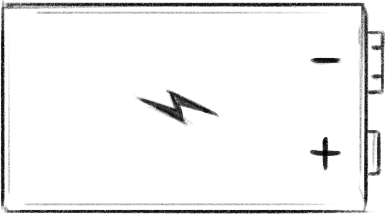
\includegraphics[width=0.25\textwidth]{images/65.png}
    } &
    \parbox[c]{0.6\textwidth}{
        \vspace*{1em}
        種類:6LR61\\
        電圧:9.0 V\\
        セル:二酸化マンガン亜鉛\\
        ホルダー:1つ
        \vspace*{1em}
    }\\ \hline
    \parbox[c]{0.3\textwidth}{
        \centering
        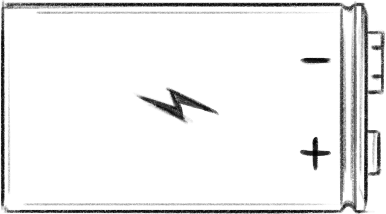
\includegraphics[width=0.25\textwidth]{images/66.png}
    } &
    \parbox[c]{0.6\textwidth}{
        \vspace*{1em}
        種類:6LS05\\
        電圧:9.2 V\\
        セル:二酸化マンガン亜鉛\\
        ホルダー:1つ
        \vspace*{1em}
    }\\ \hline
    \parbox[c]{0.3\textwidth}{
        \centering
        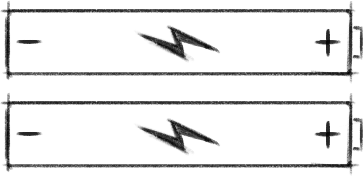
\includegraphics[width=0.25\textwidth]{images/67.png}
    } &
    \parbox[c]{0.6\textwidth}{
        \vspace*{1em}
        種類:CR61\\
        電圧:2 $\times$ 1.3 V\\
        セル:二酸化マンガンリチウム\\
        ホルダー:2つ、同じ方向
        \vspace*{1em}
    }\\ \hline
    \parbox[c]{0.3\textwidth}{
        \centering
        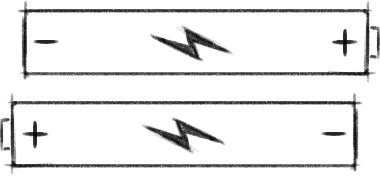
\includegraphics[width=0.25\textwidth]{images/68.png}
    } &
    \parbox[c]{0.6\textwidth}{
        \vspace*{1em}
        種類:CR61\\
        電圧:2 $\times$ 1.3 V\\
        セル:二酸化マンガンリチウム\\
        ホルダー:2つ、反対方向
        \vspace*{1em}
    }\\ \hline
    \parbox[c]{0.3\textwidth}{
        \centering
        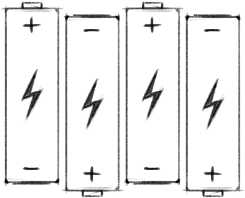
\includegraphics[width=0.25\textwidth]{images/69.png}
    } &
    \parbox[c]{0.6\textwidth}{
        \vspace*{2em}
        種類:2SF11\\
        電圧:4 $\times$ 2.0 V\\
        セル:酸化銀\\
        ホルダー:4つ、反対方向
        \vspace*{2em}
    }\\ \hline
    \parbox[c]{0.3\textwidth}{
        \centering
        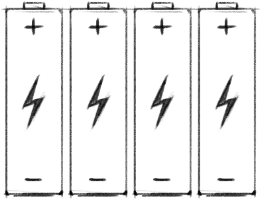
\includegraphics[width=0.25\textwidth]{images/70.png}
    } &
    \parbox[c]{0.6\textwidth}{
        \vspace*{2em}
        種類:2SF11\\
        電圧:4 $\times$ 2.0 V\\
        セル:酸化銀\\
        ホルダー:4つ、同じ方向
        \vspace*{2em}
    }\\ \hline
\end{tabular}
\end{center}



\newpage
\vspace*{\fill}

\newpage
\section*{付録II:起爆剤の種類}

TiNT博士は比較的小さな起爆剤を爆弾内に配置します。その起爆剤が主火薬を爆発させます。最も一般的な起爆剤は次のとおりです。




\bgroup
\def\arraystretch{1.3}
\begin{tabular}{|>{\centering}p{0.3\textwidth}|p{0.6\textwidth}|}
\hline
種類  & \hspace*{\fill}特性\hspace*{\fill} \\ \hline
{\Large C-4} & \begin{tabular}{@{}l@{}}主成分:RDX\\ 化学式:\ce{C3H6N6O6}\\ 化合物分類:脂肪族\\ 相対有効係数:1.6*\\ 爆発速度:8750 m/s\end{tabular} \\ \hline
{\Large Semtex} & \begin{tabular}{@{}l@{}}主成分:PETN\\ 化学式:\ce{C5H8N4O12}\\ 化合物分類:脂肪族\\ 相対有効係数:1.66*\\ 爆発速度:8400 m/s\end{tabular} \\ \hline
{\Large ダイナマイト} & \begin{tabular}{@{}l@{}}主成分:ニトログリセリン\\ 化学式:\ce{C3H5N3O6}\\ 化合物分類:脂肪族\\ 相対有効係数:1.5*\\ 爆発速度:7700 m/s\end{tabular}  \\ \hline
{\Large TNT} & \begin{tabular}{@{}l@{}}主成分:トリニトロトルエン\\ 化学式:\ce{C7H5N3O6}\\ 化合物分類:芳香\\ 相対有効係数:1.0*\\ 爆発速度:6900 m/s\end{tabular} \\ \hline
{\Large 即席爆発物}  & \begin{tabular}{@{}l@{}}主成分:TATP\\ 化学式:\ce{C9H18O6}\\ 化合物分類:脂肪族\\ 相対有効係数:0.83*\\ 爆発速度:5300 m/s\end{tabular}  \\ \hline
\end{tabular}
\egroup

* TNT 1 kgに対して


\newpage
\vspace*{\fill}

\newpage
\section*{付録III:モールス符号}

爆弾のセキュリティモジュールの多くは、モールス符号に基づいています。点は、短い光(または音)信号を表します。線は長い信号を表します。長い信号は、短い信号よりも3倍長くなります。

\vspace*{1em}

\newcommand{\dt}{\kern-0.5pt\raisebox{0.4ex}{.}}

\bgroup
\Large
\def\arraystretch{1.5}
\begin{tabular}{|p{0.3\textwidth}|p{0.3\textwidth}|p{0.3\textwidth}|}
\hline
A\quad \dt-         & M\quad --         & Y\quad -\dt-- \\ \hline
B\quad -\dt\dt\dt   & N\quad -\dt       & Z\quad --\dt\dt \\ \hline
C\quad -\dt-\dt     & O\quad ---        & 1\quad \dt---- \\ \hline
D\quad -\dt\dt      & P\quad \dt--\dt   & 2\quad \dt\dt--- \\ \hline
E\quad \dt          & Q\quad --\dt-     & 3\quad \dt\dt\dt-- \\ \hline
F\quad \dt\dt-\dt   & R\quad \dt-\dt    & 4\quad \dt\dt\dt\dt- \\ \hline
G\quad --\dt        & S\quad \dt\dt\dt  & 5\quad \dt\dt\dt\dt\dt \\ \hline
H\quad \dt\dt\dt\dt & T\quad -          & 6\quad -\dt\dt\dt\dt \\ \hline
I\quad \dt\dt       & U\quad \dt\dt-    & 7\quad --\dt\dt\dt \\ \hline
J\quad \dt---       & V\quad \dt\dt\dt- & 8\quad ---\dt\dt \\ \hline
K\quad -\dt-        & W\quad \dt--      & 9\quad ----\dt \\ \hline
L\quad \dt-\dt\dt   & X\quad -\dt\dt-   & 0\quad ----- \\ \hline
\end{tabular}
\egroup


\newpage
